\section{Geometria de Distâncias Euclidianas\label{sec:GD}}
Apresenta-se nesta seção uma introdução a \textit{Geometria de Distâncias Euclidianas}. O nome ``Geometria de Distâncias'' diz respeito ao conceito desta geometria basear-se em distâncias ao invés de pontos. A palavra ``Euclidiana'' é importante para caracterizar as arestas --- elementos fundamentais associados as distâncias --- como segmentos, sem restringir seus ângulos de incidência \cite{libertiEDG}.

\subsection{Como tudo Começou}

Por volta de 300 AC, Euclides de Alexandria organizou o conhecimento de sua época acerca da Geometria em uma obra composta por treze volumes, onde construiu, a partir de um pequeno conjunto de axiomas fortemente baseado nos conceitos de pontos e linhas, a chamada \textit{Geometria Euclidiana} \cite{elementosEuclides}. Em contraponto a visão original de Euclides, os primeiros conceitos geométricos usando \textit{apenas distâncias} costumam estar associados aos trabalhos de Heron de Alexandria (10 a 80 DC) \cite{libertiEDG}, com o desenvolvimento de um teorema que leva seu nome, como segue: 
\begin{center}
	\begin{minipage}{0.9 \linewidth}
		\textbf{\textit{Teorema de Heron}:} Sejam $s$ o \textit{semiperímetro} de um triângulo (se $p$ é o perímetro, $s = \frac{p}{2}$) e $a$, $b$ e $c$ os comprimentos dos três lados deste triangulo. Então, a área $A$ do triângulo é
		
		\begin{equation}\tag{Fórmula de Heron}
		A = \sqrt{s(s-a)(s-b)(s-c)}.
		\label{eq:heron}
		\end{equation}
	\end{minipage}
\end{center} 
Pode-se dizer que esse foi o nascimento da \textit{Geometria de Distâncias} (\textit{Distance Geometry}, ou DG).

Algumas centenas de anos depois, em 1841, Arthur Cayley (1821 a 1895) generalizou a~\ref{eq:heron} através da construção de um determinante que calcula o conteúdo (volume $n$-dimensional) de um \textit{simplex}\footnote{Um simplex é uma generalização do conceito de triangulo a outras dimensões, i.e.: O \textit{0-simples} é um ponto, \textit{1-simplex} é um segmento de reta, \textit{2-simplex} é um triangulo e o \textit{3-simplex} é um tetraedro.} em qualquer dimensão \cite{cayley1841HaronGD}. Um século depois, em 1928, o matemático austríaco Karl Menger (1902 a 1985) re-organizou as ideias de Cayley e trabalhou em uma construção axiomática da geometria através de distâncias \cite{mengerDeterminante} --- donde a alteração no nome do determinante de Cayley para como é conhecido hoje: ``\textit{Determinante de Cayley-Menger}''.  

\begin{center}
	\begin{minipage}{0.9 \linewidth}
		\textbf{Definição:} Sejam $A_0, A_1, \dots, A_n$ $n + 1$ pontos que definem os vértices de um $n$-simplex em um espaço euclidiano $K$-dimensional, onde $n\leq K$, e seja $d_{ij}$ a distância entre os vértices $A_i$ e $A_j$, onde $0\leq i < j \leq n$. Então, o conteúdo $v_n$ desse $n$-simplex é
	\end{minipage}
\end{center} 

\vspace{-0.5cm}

\begin{equation}\tag{Determinante de Cayley-Menger}
v_n^2 = \frac{(-1)^{n+1}}{(n!)^22^n}
\begin{vmatrix}
0 & d^2_{01} &  d^2_{02} & \ldots & d^2_{0n} & 1\\ 
d^2_{01} & 0 & d^2_{12} & \ldots & d^2_{1n} & 1\\ 
d^2_{02} & d^2_{12} &  0 & \ldots & d^2_{2n} & 1\\ 
\vdots & \vdots &  \vdots & \ddots & \vdots & \vdots\\ 
d^2_{0n} & d^2_{1n} & d^2_{2n}  & \ldots & 0 & 1\\ 
1 & 1 & 1  & \ldots & 1 & 0\\ 
\end{vmatrix}.
\label{determinanteCayleyMenger}
\end{equation}

Mas foi só com Leonard Blumenthal (1901 a 1984) que, em 1953, o termo Geometria de Distâncias foi cunhado --- com a publicação de seu livro \textit{``Theory and Applications of Distance Geometry''} \cite{Blumenthal:53}.
Blumenthal dedicou sua vida de trabalho para clarificar, organizar e traduzir as obras originais em alemão \cite{libertiEDG}. Ele acreditava que o problema mais importante nesta área era o \textit{``Problema de Subconjunto''} (ou \textit{Subset Problem}, originalmente), que consistia em encontrar condições necessárias e suficientes a fim de decidir quando uma matriz simétrica era, de fato, uma \textit{matriz de distâncias}\footnote{Seja o par $(\mathcal{X}, d)$ um \textit{espaço métrico} (vide Apêndice~\ref{ap:metric}), onde $\mathcal{X} = \{x_1, \dots, x_n\}$. Uma \textit{matriz de distância sobre $\mathcal{X}$} é uma matriz quadrada $D_{n\times n} = (d_{uv})$ onde, para todo $u,v \leq n$, temos $d_{uv} = d(x_u,x_v)$ \cite{carlileGDandAplications}.} \cite{carlileGDandAplications}. Uma restrição desse problema à métrica euclidiana chama-se \textit{Problema de Matrizes de Distâncias Euclidianas} (ou EDMP, do inglês \textit{Euclidean Distance Matrix Problem}), como segue definida:

\begin{center}
	\begin{minipage}{0.9 \linewidth}
		\label{EDMP}
		\textbf{Problema de Matrizes de Distâncias Euclidianas:} Determinar se, para uma dada matriz quadrada $D_{n\times n} = (d_{ij})$, existe um inteiro $K$ e um conjunto $\{p_1, \dots, p_n \}$ de pontos em $\mathbb{R}^K$ tal que $d_{ij} = \lVert p_i - p_j\rVert$ para todo $i,j \leq n$.
	\end{minipage}
\end{center} 

Condições necessárias e suficientes para que uma matriz seja, de fato, uma matriz de distância euclidiana são dados em \cite{EDMPResolucao}. Para isso, apresenta-se um teorema onde se utiliza o~\ref{determinanteCayleyMenger} na criação de duas condições afirmando que, afim de $D_{n\times n}$ ser uma matriz de distâncias euclidianas, deve haver um $K$-simplex $S$ de referência com conteúdo $v_K \neq 0$ em $\mathbb{R}^K$ e que todos os $(K+1)$-simplex e $(K+2)$-simplex contendo S como uma das faces devem estar contidos em $\mathbb{R}^K$ \cite{carlileGDandAplications}.

Blumenthal percebeu a importância em se respeitar as restrições métricas estabelecidas pelas matrizes de distâncias.
\begin{quotation}
	\textit{Quando temos como dado um conjunto de distâncias entre pares de pontos, a geometria das distâncias pode dar uma dica para encontrar um conjunto de coordenadas correto para pontos no espaço Euclideano tridimensional, satisfazendo as restrições de distâncias dadas.}
	\begin{flushright}
		(Blumenthal, 1953, \cite{Blumenthal:53})
	\end{flushright}
\end{quotation}

Pode-se dizer que resolver o Problema de Matrizes de Distâncias Euclidianas está intimamente relacionado com descobrir as coordenadas dos pontos que definem suas distâncias. Perceba que este é um problema inverso, onde o ``problema direto'' correspondente é calcular distâncias associadas a pares de pontos dados. Note que este estudo tem enorme aplicabilidade \cite{carlileGDandAplications}.
\\

Adiante, em 1979, Yemini (atualmente professor emérito de Ciência da Computação na Universidade de Columbia) foi o primeiro a flexibilizar a definição do EDMP ao considerar um conjunto de distâncias esparso \cite{Yemini:79,carlileGDandAplications} --- i.e., que não se tem todas as distâncias dadas a priori. Com isso, introduziu-se o que se chamou de \textit{Problema Posição - Localização}, onde deseja-se calcular a localização de todos os objetos imersos em um espaço geográfico \cite{Yemini:79}. 

Assim, foi possível re-formular o problema fundamental de Geometria de Distâncias, o qual pode ser caracterizado de forma mais moderna pela utilização da Teoria de Grafos \cite{carlileGDandAplications}.

\subsection{O Problema Fundamental}

Uma \textit{realização} é uma função que mapeia um conjunto de vértices de um grafo $G$ para um espaço euclidiano de alguma dimensão dada \cite{libertiEDG}.

\begin{center}
	\begin{minipage}{0.9 \linewidth}
		\textbf{Problema de Geometria de Distâncias (DGP):} Dados um grafo simples, ponderado e conectado $G = (V, E, d)$ e um inteiro $K>0$, encontre uma realização $x: V \longrightarrow \mathbb{R}^K$ tal que:
		\begin{equation}
		\forall \{u,v\} \in E, \hspace{0.5cm} \lVert x(u) - x(v) \rVert = d(u,v). \label{eq:DGP}
		\end{equation}
	\end{minipage}
\end{center}

Desde que uma realização seja encontrada, também dá-se a ela o nome de \textit{solução} do DGP. Por simplicidade --- claramente um abuso de notação ---, pode-se escrever $x_u$ e $d_{uv}$ no lugar de $x(u)$ e $d(u,v)$, respectivamente.

A principal diferença desta definição para o EDMP está acerca de que uma matriz de distância essencialmente representa um \textit{grafo ponderado completo}. Em contraponto, o DGP não empoe qualquer estrutura em $G$\footnote{A menos, é claro, no que diz respeito a seus vértices estarem conectados. Porém, caso $G$ não seja conectado, então ele consiste de um conjunto de diferentes subgrafos conectados, donde, a fim de solucionar o DGP, pode-se realizar cada subgrafo separadamente \cite{libertiEDG}.}, seguindo o conceito de matriz esparsa estabelecido por Yemini.

Por fim, na equação~\ref{eq:DGP}, utiliza-se a norma euclidiana $\lVert$ $\cdot$ $\rVert$ como métrica (ver Apêndice~\ref{ap:metric}), donde pode-se reescrever esta equação como

\begin{equation*}
	\forall \{u,v\} \in E, \hspace{0.5cm} \sqrt{\sum_{i=1}^{K}(x_{ui} - x_{vi})^2} = d_{uv}.
\end{equation*}

Como a definição de métrica garante a positividade das distâncias, pode-se esconder a raiz quadrada na equação acima, i.e.

\begin{equation}
\forall \{u,v\} \in E, \hspace{0.5cm} \sum_{i=1}^{K}(x_{ui} - x_{vi})^2 = d_{uv}^2.
\label{eq:DGPSistemaQuadratico}
\end{equation}

\subsection{Os Diferentes Problemas em DG}

Em 2014, Leo Liberti \textit{et al.} publicaram um ótimo compendio sobre a \textit{Geometria de Distâncias Euclidianas e suas Aplicações} \cite{carlileGDandAplications} e, em particular, desenvolveram um estudo  taxonômico muito interessante sobre os problemas clássicos da área. No que se segue, devido a grande quantidade de siglas e variações dentro de DG, apresenta-se parte desse estudo, visando organizar os conceitos. 
\\

As principais aplicações em DG são no \textit{calculo de estruturas moleculares} \cite{crippen:DistancesAndMolecularConformation}, na \textit{localização de sensores em rede sem fio} (\textit{Wireless Sensor Network Localization}, ou WSNL) \cite{yemini1978positioning}, em \textit{cinemática inversa} (\textit{Inverse Kinematic}, ou IK) \cite{cinematicaInversa} e em \textit{escalonamento multidimensional} (\textit{Multidimensional Scaling}, ou MDS) \cite{multidimensionalScaling}.

\subsubsection{Conformações Moleculares}

Existe uma relação muito forte com a forma geométrica das moléculas e suas funções em organismos vivos \cite{bioquimicaLehninger}. Projetar drogas para curar uma doença específica se trata basicamente de conhecer o que uma certa proteína pode fazer em um organismo \cite{libertiEDG}. Proteínas se ligam em outras moléculas através do equilíbrio de forças agindo entre elas\footnote{Ou seja, o equilíbrio da energia potencial das moléculas, proporcional, principalmente, as variações nos comprimentos das ligações covalentes, as variações nos ângulos entre duas ligações covalentes consecutivas, as rotações sobre as ligações covalentes e as interações de van der Waals e interações eletrostáticas entre átomos \cite{carlileTese}.}, por tanto, suas ligações dependem do seu formato. 

Proteínas são constituídas por um grande conjunto de átomos e, alguns pares destes, trocam ligações químicas --- sabe-se quais são esses átomos através de experimentos de cristalografia \cite{ramachandran1974MolStructure}. Então, se os átomos de uma molécula forem rotulados da forma $1,3,4,\dots,n$, então é possível inferir: 
\begin{itemize}
	\item O conjunto de ligações $\{u,v\}$, onde $u,v$ são átomos em $\{1,\dots,n\}$;
	\item A distância entre $u$ e $v$ (para cara par ligado);
	\item O ângulo interno $\theta_v$ definido por duas ligações $\{u,v\}$ e $\{v,w\}$, com um átomo $v$ em comum.
\end{itemize} 

Além desses dados, também é possível obter informações a partir de experimentos mais sofisticados, como a \textit{Ressonância Magnética Nuclear} (RMN). Neste experimento é escolhida uma faixa de radiofrequência para bombardear uma amostra que está imersa em um campo magnético bastante intenso. Dependendo da radiofrequência utilizada (costuma-se usar a do hidrogênio), alguns núcleos atômicos irão absorver energia e outros não. Caso atinja-se uma frequência exata de ressonância dentro destes núcleos atômicos, é possível medir essa ressonância como um sinal de radiofrequência enviado dos núcleos atômicos --- para calcular distâncias entre átomos próximos, com distâncias menores que 5\AA.

De posse dessas informações, deseja-se realizar (localizar) todos os átomos da molécula. Esse problema, com todas as informações moleculares disponíveis, denomina-se \textit{Estrutura Proteica a partir de Dados Brutos} (\textit{Protein Structure from Raw Data}, ou PSRD)

Em particular, como as coordenadas atômicas pertencem ao $\mathbb{R}^3$, há uma particularização do DGP para o caso molecular, chamado \textit{Problema de Geometria de Distâncias Moleculares} (\textit{Molecular DGP}, ou MDGP). Trata-se do DGP com $K = 3$ fixo.

\subsubsection{Localização de Sensores}

O \textit{Problema de Localização de Sensores em Rede sem Fio} (ou \textit{WSNL Problem}) surge quando é necessário localizar um conjunto de objetos equipados com sensores eletrônicos capazes de medir distâncias entre si, geograficamente distribuídos, usando apenas medidas de distâncias entre pares destes objetos \cite{yemini1978positioning}. 

Por exemplo, \textit{smartphones} com WIFI ativo podem criar uma rede conhecida por \textit{Rede Ad-Hoc}, \textit{i.e.}, eles conseguem criar uma rede para comunicar-se entre si, de forma \textit{peer-to-peer}, sem a necessidade de uma torre central --- cada aparelho funciona como uma pequena torre, de forma que a distância entre os aparelhos não pode ser excessiva.
Dessa forma, os \textit{smartphones} podem estimar a distância $r$ de emparelhamento das suas conexões ao medir, por exemplo, qual a potência de transmissão do sinal, uma vez que sabe-se que a potência $P$ de uma transmissão eletromagnética cai da forma 
\begin{equation}
	P = \frac{X}{r^n},
\end{equation}
onde $X$ e $n$ são constantes e dependem muito das condições do experimento, sendo obtidas experimentalmente \cite{savvides2001dynamic}.

Em essência, um problema do tipo WSNL segue a mesma definição do DGP, porém, com um subconjunto $A\subset V$ de vértices (chamados \textit{âncoras}), onde os elementos de $A$ tem uma posição em $\mathbb{R}^k$ dada a priori --- isso é feito pois, normalmente, interessa saber a posição relativa de um objeto a outro, como é o caso do Sistema de Posicionamento Global, onde temos os satélites como âncoras e desejamos saber a posição dos aparelhos GPS em relação aos satélites.

Por motivos práticos --- semelhantes ao caso molecular --- as variações de interesse desse problema tem o $K$ fixo em $K= 2$ ou $K=3$. É comum, também, que se defina um WSNL como \textit{solucionável} somente se seu grafo possua uma única realização válida \cite{libertiEDG} --- noção conhecida como \textit{globalmente rígido}: Diz-se que um grafo é \textit{globalmente rígido} quando ele possui uma realização genérica $x$ e, para todas as outras realizações $x'$, $x$ é congruente a $x'$. 

\subsubsection{Dinâmicas em Cinemática Inversa}

Muito utilizada em robótica e animação computadorizada, a cinemática inversa cerne sobre mecanismos e seus movimentos rígidos, onde restringe-se os movimentos de forma a preservar a geometria do sistema. Sem o auxilio computacional e matemático a manipulação de mecanismos com muitos graus de liberdade  pode ser inviável: Imagine a manipulação manual de cem vértices em uma haste simulando o comportamento de um braço articulado em uma animação. Com o auxílio da DG, um animador pode apenas configurar a posição final de um pequeno grupo de vértices (como os da extremidade da aresta, por exemplo) e um algorítimo de cinemática inversa é capaz de verificar se aquela posição é ou não viável e, se viável, qual a realização de todo o conjunto de vértices em razão da posição configurada \cite{cinematicaInversa}.

Visando tal restrição mecânica, define-se o \textit{Problema de Cinemática Inversa} (\textit{Inverse Kinematic Problem}, ou IKP) como uma variação do WSNL --- logo, tem o objetivo de descobrir posições em relação a certos pontos previamente realizados --- com uma restrição no grafo que define o problema: deve ser um caminho simples com seus vértices finais sempre sendo âncoras \cite{carlileGDandAplications}.

\subsubsection{Escalonamento Multidimensional}

O problema de \textit{Escalonamento Multidimensional} (\textit{Multidimensional Scaling}, ou MDS)
é definido como \cite{carlileGDandAplications}: Dado um conjunto $X$ de vetores, encontre um conjunto $Y$ de vetores com menor dimensão (com $|X| = |Y|$) tal que a distância entre cada $i$-ésimo e $j$-ésimo vetores de $Y$ tenham, aproximadamente, a mesma distância que seus pares de vetores correspondentes em $X$.

Esse problema é muito aplicado na analise de dados em Big Data \cite{libertiEDG}. É um meio de facilitar a visualização do nível de similaridade entre casos individuais --- que não necessariamente precisam ter uma conexão aparente --- em um conjunto de dados. Pode-se usá-lo, por exemplo, para visualizar em uma escala bidimensional ($\mathbb{R}^2$) a evolução da locomoção de animais no espaço tridimensional utilizando dados de séries temporais (espaço em diferentes tempos, logo, dados em $\mathbb{R}^4$).

\subsection{A Busca de uma Solução}

A abordagem mais simples, pode-se pensar, para encontrar um conjunto de soluções que satisfação a equação~\ref{eq:DGPSistemaQuadratico} é resolver o sistema de equações diretamente \cite{carlileBook31Coloquio}. Infelizmente, para $K \geq 2$, há evidencias de que uma solução de forma fechada onde todo componente de $x$ é expresso por raízes, não é possível \cite{libertiEDG}. 

No entanto, pode-se re-formular o problema como um problema de otimização global \cite{libertiEDG}, onde o objetivo é minimizar a soma dos \textit{erros}\footnote{Em otimização, vê-se a equação~\ref{eq:DGP} de forma não exata: $\lVert x_u - x_v \rVert = d_{uv} + \varepsilon$, onde $\varepsilon$ é chamado \textit{erro}. Ou seja, para minimizar o erro, precisa-se minimizar a expressão $f(x_u,x_v) = \lVert x_u - x_v \rVert - d_{uv}$.} entre as distâncias dadas a priori e as calculadas. Para isso, pode-se considerar uma única expressão que englobe todos os $n$ erros, da forma
\begin{equation}
	f(x_1,\dots,x_n) = \sum_{(i,j)\in E} \left(\lVert x_i - x_j \rVert - d_{ij}\right)^2.
\end{equation}

Fica claro que encontrar uma solução para o DGP é equivalente a encontrar realizações $x_i \in \mathbb{R}^3$, $i=1,\dots,n$, se e somente se $f(x_1,\dots,x_n) = 0$ \cite{libertiEDG}. Pela definição de métrica (vide Apêndice~\ref{ap:metric}), 0 é o menor valor possível para $f$, donde diz-se que deseja-se \textit{minimizar a função} $f: \mathbb{R}^n \longrightarrow \mathbb{R}$ \cite{carlileBook31Coloquio}. Ou seja,
\begin{equation}
	\min_{x_i \in \mathbb{R}^n} f(x_1,\dots,x_n).
\end{equation}

E, no caso da métrica euclidiana (vide Apêndice~\ref{ap:metric}), temos

\begin{equation}
 \min_{x_j \in \mathbb{R}^n} \sum_{(u,v)\in E} \left(\sum_{i=1}^{K}(x_{ui} - x_{vi})^2 - d_{uv}^2\right)^2.
 \label{eq:DGPminEuclid}
\end{equation}

Por tanto, a equação~\ref{eq:DGPminEuclid} tem como objetivo a minimização de um polinômio de múltiplas variáveis de grau quatro. 
\\

Um dos desafios da Otimização Global é que muitos dos métodos existentes --- em especial, os mais eficientes --- não garantem que uma otimização \textit{global} será encontrada \cite{libertiEDG}. Isso se dá pois, dependendo do comportamento da função, existem muitos ótimos locais e os métodos não conseguem diferenciá-los de um global. %Em DG, a distribuição geométrica dos vértices do grafo está intimamente ligada com o comportamento da função objetivo --- donde, por exemplo, em WSNL, é interessante o estudo da distribuição geométrica dos sensores afim de melhorar a busca por ótimos globais \cite{eren2004rigidity}.

Infelizmente, essa abordagem via otimização é custosa do ponto de vista computacional \cite{libertiEDG}. Saxe demonstrou em 1979 \cite{Saxe:79} que resolver um DGP para qualquer dimensão --- i.e., para qualquer valor de $K$ --- tem a complexidade computacional da classe \textbf{NP}-Hard. Em outras palavras, isso significa que a quantidade de mínimos locais de um DGP cresce exponencialmente proporcional a $|V|$ \cite{carlileIntroductionMDGP}. 

\subsubsection{A Quantidade de Soluções do Problema}
Dada uma solução de um DGP, obtêm-se facilmente uma quantidade infinita (não enumerável!) de outras realizações válidas, distintas, através de rotações e translações desta solução inicial \cite{carlileBook31Coloquio}, devido ao fato destes movimentos serem rígidos, donde não deformam as distâncias associadas aos pares de vértices. Por descreverem uma mesma geometria, essa realizações não são interessantes. Contudo, se for desconsiderado essas redundâncias, a quantidade de soluções do DGP depende da estrutura geométrica do grafo que a define: (i) podem não haver nenhuma realização; (ii) uma única realização; (iii) uma quantidade finita (não única) de realizações; ou, (iv) um número incontável de realizações \cite{libertiEDG}. Perceba que, curiosamente, a quantidade de soluções de um DGP somente não pode ser um número infinito e enumerável --- sabe-se isso através de estudos em \textit{Geometria Algébrica Real} \cite{benedettireal}.\\
 
Ou seja, supondo que o conjunto solução de um DGP seja não vazio, sabe-se que ele é não enumerável ou finito. Se for finito (normalmente o caso desejado), além de aplicar os métodos de Otimização Global --- já definidos como custosos computacionalmente ---, pode-se explorar outras abordagens, como a Otimização Combinatória \cite{carlileBook31Coloquio}. 

\subsection{Combinatória do DGP}

Nesta seção, estuda-se sobre as condições que garantem a finitude do conjunto solução do problema ao analisar o espaço de busca por uma solução. Em particular, para um DGP definido em um espaço de dimensão $K$, apresenta-se uma classe de grafos com propriedades muito interessantes: dos $(K+2)$-cliques, ou seja, dos grafos completos com dois vértices a mais do que o número de dimensões do seu espaço.

\subsubsection{Realização de Grafos Completos}

 Dado um $(K+1)$-clique com vértices não coincidentes (essa condição ficará mais clara ao decorrer desta seção), sabe-se que \textit{se ele possui} uma realização em $\mathbb{R}^{K-1}$, \textit{ela é única} a menos de rotações e translações \cite{libertiEDG, hendrickson1992conditions, connelly1991generic}. Porém, visto que para solucionar um DGP interessa uma solução em $\mathbb{R}^K$ ao invés de $\mathbb{R}^{K-1}$, pode-se usar um corolário um tanto óbvio da afirmação anterior: um $(K+2)$-clique com vértices não coincidentes tem, no máximo, uma realização única no espaço $\mathbb{R}^K$ (novamente, \textit{única} a menos de movimentos rígidos). 

Por tanto, dependendo da estrutura do grafo que define um DGP (em especial, dependendo de sua rigidez \cite{eren2004rigidity, alfakihEuclideanDistanceMatricesApplicationsRigidity}), obter uma solução do problema pode garantir a unicidade desta solução. Essa característica é de fundamental importância para algumas classes de problemas em DG, como o caso da WSNL, onde somente realizações únicas são consideradas como soluções. Ainda assim, é preciso apresentar um método para obter uma solução.  É o que se faz a seguir, baseado em \cite{libertiEDG} e \cite{trilaterationDong}. 
\\

Considere um 3-clique ponderado com $V = \{1,2,3\}$, onde $d_{12} = d_{23} = 1$ e $d_{13} = 2$. Então, uma possível realização sobre a reta real $\mathbb{R}$ que satisfaça todas as distâncias é $x_1 = 0$, $x_2 = 1$ e $x_3 = 2$. Uma forma de obter o valor de $x_3$, dado os valores de $x_1$ e $x_2$ e as distâncias $d_{13}$ e $d_{23}$, é a \textit{trilateração}.

\subsubsection{Trilateração\label{sec:trilateration}}

 Sabendo que $d_{13} = \lVert x_3 - x_1\rVert = 2$ e $d_{23} = \lVert x_3 - x_2 \rVert = 1$ e que, usando a norma euclidiana\footnote{Ver Apendixe~\ref{ap:metric}}, $\lVert u-v\rVert^2 = (u-v)^2 = u^2 -2uv + v^2$, tem-se

\begin{equation}
	x_3^2 - 2x_1x_3 +x_1^2 = 4 \quad \textrm{e}
	\label{eq:trilateration1}
\end{equation}
\begin{equation}
x_3^2 - 2x_2x_3 +x_2^2 = 1. \quad
\label{eq:trilateration2}
\end{equation}

Subtraindo a equação~\ref{eq:trilateration2} da~\ref{eq:trilateration1}, obtêm-se

\begin{equation*}
	2(x_1-x_2)x_3 = x_1^2 - x_2^2 - 3 \ \Rightarrow \ 2x_3 = 4 \ \Rightarrow \ x_3 = 2.
\end{equation*}

Pode-se generalizar esse exemplo facilmente para $(K+2)$-cliques em $\mathbb{R}^{K}$ \cite{libertiEDG}: Precisa-se conhecer a posição de $K+1$ vértices e as distâncias destes ao $(K+2)$-ésimo vértice, assim, pode-se realizar o $(K+2)$-ésimo vértice, em tempo linear, resolvendo um sistema de $K+1$ equações como acima.
\\

Isto é, sejam $x_1, \dots, x_{k+1} \in \mathbb{R}^{K}$ as posições para $K+1$ vértices de um $(K+2)$-clique e, para todo $j\leq K+1$, seja $d_{j,K+2}$ a distância associada com a aresta $\{j, K+2\}$. Seja $y \in \mathbb{R}^{K}$ a posição do $(K+2)$-ésimo vértice; então, $y$ deve respeitar as $K+1$ equações quadráticas $\forall j\leq K+1$, $\lVert x_j-y\rVert^2 = d_{j,K+2}^2$, com $K$ incógnitas  $y_1, \dots,y_{K}$:

\begin{equation}
	\begin{cases} 
		\lVert y \rVert^2 -2x_1y + \lVert x_1\rVert^2 \ = \ d^2_{1,K+2}
		\\
		\qquad\qquad\qquad\quad\qquad \!\vdots
		\\
		\lVert y \rVert^2 -2x_{K+1}y + \lVert x_{K+1}\rVert^2 \ = \ d^2_{K+1,K+2}
	\end{cases}
	\label{eq:DGPsistemaEquacoes1}
\end{equation}

Para qualquer $h\leq K+1$, seja $e_h$ a $h$-ésima equação no sistema de equações~\ref{eq:DGPsistemaEquacoes1}: tomando todo $h<K+1$, pode-se obter as $K$ diferenças $(e_h-e_{K+1})$ e formar um novo sistema,  contendo $K$ equações com $K$ incógnitas:

\begin{equation}
\begin{cases} 
2(x_1-x_{K+1}) \;\cdot y \ = \ \lVert x_1\rVert^2 - \lVert x_{K+1}\rVert^2 - d^2_{1,K+2} + d^2_{K+1,K+2} 
\\
\qquad\qquad\qquad\qquad\!\!\!\vdots
\\
2(x_{K}-x_{K+1}) \cdot y \ = \ \lVert x_{K}\rVert^2 - \lVert x_{K+1}\rVert^2 - d^2_{K,K+2} + d^2_{K+1,K+2} 
\end{cases}
\label{eq:DGPsistemaEquacoes2}
\end{equation}
\\

Note que o sistema de equações~\ref{eq:DGPsistemaEquacoes2} é um \textit{sistema linear} da forma 
\begin{equation}
	Ay=b,
	\label{eq:DGPLinearSystem}
\end{equation}
onde $A = (2a_{ij})$ é uma matriz quadrada $K \times K$ com $a_{ij} = x_{ij} - x_{K+1j}$ para todo $i,j \leq K$, e $b = (b_1, \dots, b_{K})^T$ com $b_i = \lVert x_i\rVert^2 - \lVert x_{K+1}\rVert^2 - d^2_{i,K+2} + d^2_{K+1,K+2}$ para todo $i\leq K$. 
\\

Diferentes métodos para solução de sistemas lineares como a equação~\ref{eq:DGPLinearSystem} são encontrados na bibliografia \cite{AlgebraLinearElon} --- no geral, a escolha do melhor depende de propriedades da matriz $A$, como sobre sua esparsidade. Em especial, se $A$ não é uma matriz singular, então ela possui uma inversa $A^{-1}$. Pode-se, por tanto, obter a posição do $(K+2)$-ésimo vértice fazendo

\begin{equation}
	Ay = b \quad \Rightarrow \quad A^{-1}Ay = A^{-1}b \quad \Rightarrow \quad y = A^{-1}b = x_{K+2}.
\end{equation}
\\

No entanto, se A é singular, isso quer dizer que as linhas $a_i = x_i - x_{K+1}$ (para $i\leq K$) não são todas linearmente independentes \cite{AlgebraLinearElon}. Essa situação mostra algumas propriedades geométricas interessantes \cite{libertiEDG}. Por exemplo, se $K=1$, significa que $x_1 - x_2 = 0 \ \Rightarrow \  x_1 = x_2$, ou seja, que o segmento entre $x_1$ e $x_2$ é um simples ponto. Como estamos imersos no $\mathbb{R}^{K} = \mathbb{R}$ (i.e., a reta real), geometricamente, a situação é que ou $x_3$ está posicionado a direita ou a esquerda de $x_1 = x_2$, mas não se pode escolher. Não obstante, se $K = 2$, a singularidade de $A$ implica que o triangulo definido por $x_1$, $x_2$ e $x_3$ é apenas um segmento no plano (caso o rank de $A$ é 1) ou um simples ponto (caso o rank for 0). No primeiro caso, $x_4$ pode estar posicionado em ambos os lados da linha que contém o segmento e, no segundo caso, $x_4$ pode estar em qualquer um dos pontos formados pela circunferência com centro $x_1 = x_2 = x_3$ e raio $d_{14} = d_{24} = d_{34}$. 
Essa característica geométrica vale para valores maiores de $K$: a singularidade de $A$ está relacionada a existência de vértices coincidentes e implica que há sempre múltiplas soluções para $x_{K+2}$.\\

Por fim, é importante mencionar que a partir da equação~\ref{eq:DGPsistemaEquacoes1} podemos chegar no sistema linear~\ref{eq:DGPLinearSystem}, mas a volta não é verdadeira. Em particular, se o sistema~\ref{eq:DGPsistemaEquacoes1} tem uma solução, então o sistema~\ref{eq:DGPLinearSystem} tem a mesma solução. Porém, mesmo que o sistema~\ref{eq:DGPsistemaEquacoes1} não tenha solução, o sistema~\ref{eq:DGPLinearSystem} sempre terá uma solução única --- desde que $A$ não seja singular \cite{libertiEDG}. Sendo assim, para verificar a factibilidade de uma solução $x_{K+2}$ advinda do sistema linear~\ref{eq:DGPLinearSystem}, deve-se verificar se as distâncias aos $K+1$ vértices foram respeitadas --- ou seja, se $\lVert x_i -x_{K+2} \rVert = d_{i,K+2}$, para todo $i\leq K+1$. 
\\

\subsubsection{Devagar e Sempre}

Utilizando o método da trilateração apresentado, é possível descobrir a posição de apenas um vértice de um grafo completo. No entanto, como o objetivo é uma realização total do grafo, a seguir relembra-se uma característica dos grafos completos que contorna essa limitação de uma forma engenhosa.
\\

Seja o primeiro grafo completo da Figura~\ref{fig:grafoCompleto} formado pelo conjunto de vértices $\{v_1,v_2,v_3,v_4\}$. Perceba que esse é um 4-clique e, ao removermos o vértice $v_4$, obtemos um $3$-clique formado pelo conjunto de vértices restantes $\{v_1,v_2,v_3\}$ (no centro da Figura~\ref{fig:grafoCompleto}). Caso for retirado o vértice $v_3$ desse 3-clique, obtemos o 2-clique formado por $\{v_1, v_2\}$ (ultimo grafo da Figura~\ref{fig:grafoCompleto}). 

\begin{figure}[H]
	\begin{center}
		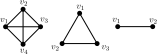
\includegraphics[width=0.55\linewidth]{secGD/figures/grafoCompleto.png}
	\end{center}
	\caption{Em ordem: 4-clique; 3-clique; 2-clique.}
	\label{fig:grafoCompleto}
\end{figure}

Perceba a existência de uma estrutura recursiva nos grafos completos, que se mantém para o caso geral: Sejam $G_{K+1} = \{V_G, E_G\}$ um $(K+1)$-clique e $v \in V_G$ um vértice qualquer de $G_{K+1}$, sempre pode-se obter um $K$-clique como o subgrafo induzido $\langle V_G \setminus \{v\}\rangle$. Isto é, se $(V,E)$ é um grafo completo, dado qualquer grafo induzido $\langle V'\rangle$ com $V'\subset V$, o subgrafo $\langle V' \rangle$ também é completo. Por conta disso, podemos utilizar essas estruturas como ``blocos básicos de construção'' para planejar uma realização iterativa do grafo como um todo, usando a trilateração para realizar um novo vértice em cada iteração. 




\subsubsection{Realização Iterativa de Grafos Completos}

A seguir, apresenta-se um algorítimo para realizar em $\mathbb{R}^K$ todos os $n$ vértices de um $(n,\frac{n^2 -n}{2})$-grafo completo $G$, com $n > K$, tendo como entrada a posição dos $(K+1)$ primeiros vértices também em $\mathbb{R}^{K}$.
\\

Primeiro, assume-se que exista um $(K+1)$-clique $G_o \subset G$, chamado clique inicial, que conhecemos a realização --- em WSNL, por exemplo, comumente se utiliza nós ancoras como clique inicial \cite{eren2004rigidity, savvides2001dynamic}. Sem perda de generalidade, seja $\{1,\dots,K+1\}$ o conjunto dos vértices que formam a clique inicial $G_o$, com realizações $\{x_1, \dots,x_{K+1}\}$. Seja, também, $N(i)$ o conjunto de vértices adjacentes ao $i$-ésimo vértice. Então, pode-se encontrar uma realização total de $G$ através do Algorítimo~\ref{alg:realizacaoIterativa}. 
\\

\begin{algorithm}[H]
	\label{alg:realizacaoIterativa}
	\tcp{Realize os próximos vértices iterativamente}
	\For{$i\in \{K+2,\dots,n\}$}{
		\tcc{Utilize o $(K+1)$-clique dos $(K+1)$ antecessores imediatos de $i$ para calcular a realização $x_i$. Caso não haja solução, atribuir $\emptyset$}
		$x_i =$ Trilateracao$(x_{i-K-1},\dots,x_{i-1})$\;
		\tcp{verifique se $x_i$ é factível com relação as demais distâncias}
		\For{$\{j\in N(i)\ ; \ j<i\}$}{
			\If{$\lVert x_i - x_j\rVert \ne d_{ij}$}{
				\tcp{Sinalizar como não factível e sair do loop}
				$x_i = \emptyset$\;
				\textbf{break}\;
			}
		} 
		\If{$x_i = \emptyset$}{
			\tcp{Retornar que a realização não é factível}
			\textbf{return} $\emptyset$\;
		}
	}
	\tcp{Retornar a realização factível}
	\textbf{return} $x$\;
	\caption{$x =$ RealizacaoIterativa$(G,d, K, x)$ \cite{libertiEDG}}
\end{algorithm}
\vspace{0.5cm}
Note que o Algorítimo~\ref{alg:realizacaoIterativa} tem a complexidade de seu pior caso como $O(K^3n)$, i.e., para todos os $n$ vértices, deve-se resolver um sistema linear $K\times K$ (trilateração). Se não existir realização factível para $G$ em $\mathbb{R}^K$, Algorítimo~\ref{alg:realizacaoIterativa} retorna $\emptyset$.

Esse processo de trilateração em $\mathbb{R}^K$ é chamado $K$-\textit{lateração} \cite{eren2004rigidity, libertiEDG}.

\subsubsection{Sobre o clique inicial $G_o$ e unicidade \label{sec:go}}
O Sistema de Posicionamento Global (GPS,  \cite{gps}) é um exemplo de WSNL que utiliza da trilateração para descobrir a localização dos aparelhos de GPS (sensores móveis). Como o objetivo é encontrar posições no $\mathbb{R}^3$, precisa-se de 4 vértices âncoras para compor o clique inicial $G_o$, que, no caso, é formado por um conjunto de satélites com posições bem conhecidas. Fica claro que, em algumas aplicações, a quantidade de vértices necessários no clique inicial pode significar um projeto de engenharia bastante custoso.

Além disso, em um primeiro momento pode parecer pouco razoável necessitar da realização prévia do clique inicial $G_o$. De fato, se o problema possuir apenas $K+1$ vértices, essa solução não faz sentido. Felizmente, em geral, os problemas de estudo costumam ser maiores \cite{carlileGDandAplications}. 
\\

Bem, como dito anteriormente, na trilateração, a necessidade de se usar um vértice a mais do que a dimensão do espaço de realização está relacionada com a unicidade da solução \cite{hendrickson1992conditions, connelly1991generic}. Perceba, os $K+1$ vértices do clique inicial mais o vértice a se realizar induzem um simplex no espaço $\mathbb{R}^K$ que, garantida a desigualdade triangular, possui um volume $K$-dimensional $\geq 0$ diretamente proporcional ao determinante de Cayley-Menger. Caso esse volume for zero, que é o que acontece com $(K+2)$-simplex em $\mathbb{R}^K$, tem-se o chamado \textit{simplex achatado} (flat simplex) com no máximo uma solução \cite{libertiEDG} (como ilustra a Figura~\ref{fig:flatsimplices}, a direita).

\begin{figure}[H]
	\begin{center}
		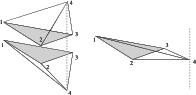
\includegraphics[width=0.7\linewidth]{secGD/figures/flatsimplices.png}
	\end{center}
	\caption{Note que as duas realizações de um mesmo $4$-clique em $\mathbb{R}^3$ (esquerda) são possíveis por respeitarem as distâncias entre os vértices, mas somente uma realização é possível em $\mathbb{R}^{2}$ (direita) \cite{libertiEDG}.}
	\label{fig:flatsimplices}
\end{figure}

Em particular, a noção que estuda a unicidade de uma realização é a de rigidez: diz-se que um grafo é \textit{globalmente rígido} se ele tem uma realização genérica $x$ e, para todas todas as outras realizações $x'$, $x$ é \textit{congruente} a $x'$ (veja Apêndice~\ref{ap:rigid}). Um grafo globalmente rígido tem solução única \cite{carlileGDandAplications, rigidezGrafosEAplicacoesAnaCarlile}.

\subsubsection{Realizando grafos $K$-laterativos em $\mathbb{R}^K$ \label{sec:oi}}

No Algorítimo~\ref{alg:realizacaoIterativa}, fica implícita a existência de uma ordem no conjunto de vértices $V$ do grafo $G$. Se $G$ é completo, de fato, qualquer ordem $(v_1,\dots,v_n)$ em $V$ é tal que $v_i$ é adjacente a todos os seus predecessores --- isto é, para todo $i>K+1$, tem-se no mínimo os $K+1$ predecessores necessários para a trilateração. Por outro lado, $G$ não precisa ser necessariamente completo para garantir isso \cite{libertiEDG}.

\begin{center}
	\begin{minipage}{0.93 \linewidth}
		\textbf{Definição:} Se $<$ é uma ordem sobre $V$ e $v\in V$ é um vértice qualquer, então $\rho(v)$ é a posição de $v$ em relação a $<$ e $\gamma(v)$ é o conjunto de predecessores de $v$ em relação a $<$. Dado um grafo $G=(V,E)$, uma ordenação $<$ sobre $V$ é chamada \textit{ordem de $K$-lateração} se:
		\begin{enumerate}
			\vspace{-0.2cm}
			\item os primeiros $K+1$ vértices de $<$ induzirem um $(K+1)$-clique $G_o$ em $G$;
			\vspace{-0.2cm}
			\item todo vértice $v$, com $\rho(v) > K+1$, tem $\lvert N_G(v) \bigcap \gamma(v)\rvert \geq K+1$.
		\end{enumerate}
	\end{minipage}
\end{center}

Um grafo $G = (V,E)$ é dito \textit{$K$-laterativo} se há uma ordem de $K$-lateração sobre $V$ associada a $G$. Perceba que um grafo $K$-laterativo não precisa ser completo e, mesmo assim, ainda é possível aplicar a trilateração em todo vértice $v \in V$, com $\rho(v) >K+1$ seguindo a ordem de $K$-lateração, pois esta garante que sempre existirá um $(K+1)$-clique realizado adjacente a $v$. O que nos leva ao enunciado principal dessa seção:

\begin{center}
	\begin{minipage}{0.93 \linewidth}
		\textbf{Teorema:} Um grafo $K$-laterativo em $\mathbb{R}^K$ é genericamente globalmente rígido em $\mathbb{R}^K$ \cite{eren2004rigidity,carlileGDandAplications}. Ou seja, se possuir realização, ela é única.
	\end{minipage}
\end{center}

A partir desses conceitos, no que se segue define-se uma subclasse do problema central e uma adaptação do Algorítimo~\ref{alg:realizacaoIterativa} para solucioná-lo.
\begin{center}
	\begin{minipage}{0.93 \linewidth}
		\textbf{O Trilaterativo DGP (TDGP):} Um DGP $(G,d,K)$ é chamado \textit{Trilaterativo DGP} se uma ordem de $K$-lateração sobre $G$ for dada.
	\end{minipage}
\end{center}

Dado um TDGP $(G,d,K)$, seja $\{x_1, \dots,x_{K+1}\}$ o conjunto de realizações dos primeiros $K+1$ vértices em relação a ordem de $K$-lateração. Uma realização $x$ de $G$ em $\mathbb{R}^K$ pode ser encontrada (ou mostrada que não existe) pelo Algorítimo~\ref{alg:realizacaoTrilateration}.
\\

\begin{algorithm}[H]
	\label{alg:realizacaoTrilateration}
	\For{$i\in \{K+2,\dots,n\}$}{
		\tcp{Procure os primeiros $K+1$ predecessores adjacentes}
		sejam $U \subset \lvert N_G(v) \bigcap \gamma(v)\rvert$, com $\lvert U\rvert = K+1$, e $W = \{x_j\ |\ j\in U\}$
		
		\tcp{Utilize o $(K+1)$-clique definido por $W$ para realizar $x_i$}
		$x_i =$ Trilateracao$(W)$\;
		\For{$\{j\in \{(N_G(v) \bigcap \gamma(v)) \setminus U\} \ ; \ j<i\}$}{
			\If{$\lVert x_i - x_j\rVert \ne d_{ij}$}{
				$x_i = \emptyset$\;
				\textbf{break}\;
			}
		} 
		\If{$x_i = \emptyset$}{
			\textbf{return} $\emptyset$\;
		}
	}
	\textbf{return} $x$\;
	\caption{$x =$ RealizacaoTrilaterativa$(G,d, K, x)$, adaptado de \cite{libertiEDG}}
\end{algorithm}
\vspace{0.4cm}

Perceba que há três características que fazem desta uma boa solução para instâncias WSNL: (i) O $(K+1)$-clique inicial necessita de uma realização dada a priori; (ii) sempre possuirá ou nenhuma (se não existe realização em $\mathbb{R}^K$), ou exatamente uma solução; (iii) é resolvido em tempo polinomial \cite{libertiEDG}.

